% \section{Methodology}
\section{Metodología}

% Define custom colors for the workflow diagram
\definecolor{datafill}{HTML}{E3F2FD}
\definecolor{datastroke}{HTML}{2196F3}
\definecolor{subsetfill}{HTML}{E0F2F1}
\definecolor{subsetstroke}{HTML}{009688}
\definecolor{processfill}{HTML}{F5F5F5}
\definecolor{processstroke}{HTML}{9E9E9E}
\definecolor{gwasfill}{HTML}{E8F5E9}
\definecolor{gwasstroke}{HTML}{4CAF50}
\definecolor{postfill}{HTML}{FFF3E0}
\definecolor{poststroke}{HTML}{FF9800}
\definecolor{vizfill}{HTML}{F3E5F5}
\definecolor{vizstroke}{HTML}{9C27B0}

% =============================
% FLUJO DE TRABAJO COMPLETO
% =============================
\begin{frame}{Flujo de trabajo completo}
  \begin{columns}[c]
    % --- WORKFLOW DETAILS ---
    \begin{column}{0.45\textwidth}
      % --- Text --- 
      {\footnotesize\sffamily
        \begin{itemize}
          \item<2-> \textcolor{datastroke}{\textbf{Datos de entrada:}} Mismos fenotipos y genotipos (imputados y arreglos chip) que el semestre pasado.
          \item<3-> \textcolor{subsetstroke}{\textbf{Diseño experimental para comparaciones:}} Asegurar \textit{independencia} estadística entre $\hat{\delta}$ y $\hat{\beta}$ usando \textbf{individuos no emparentados} (unrelated).
          \item<4-> \textcolor{gwasstroke}{\textbf{GWAS:}} FGWAS ($\hat{\delta}$) con \textit{snipar} \parencite{young2022-fgwas,guan2025-fgwas} y GWAS ($\hat{\beta}$) con REGENIE \parencite{mbatchou2021-regenie}.
          \item<5-> \textcolor{poststroke}{\textbf{Análisis posteriores:}} Correlación entre estimadores con \textit{snipar} \parencite{young2022-fgwas} y heredabilidad/correlaciones genéticas con LDSC \parencite{bulik-sullivan2015-ldsc}.
        \end{itemize}
      }
    \end{column}

    % --- COMPLETE WORKFLOW DIAGRAM ---
    \begin{column}{0.55\textwidth}
      \centering
      \resizebox{!}{5.5cm}{
        \begin{tikzpicture}[
            box/.style={rectangle, thick, rounded corners, align=center, minimum height=0.8cm, inner sep=0.2cm},
            data/.style={box, fill=datafill, draw=datastroke},
            subset/.style={box, fill=grayfill, draw=graystroke},
            process/.style={box, fill=aquafill, draw=aquastroke},
            gwas/.style={box, fill=greenfill, draw=greenstroke},
            post/.style={box, fill=yellowfill, draw=yellowstroke},
            viz/.style={box, fill=purplefill, draw=purplestroke},
            arrow/.style={->, thick, >=stealth, draw=gray!80!black}
          ]
          
          % Nodes
          \node[data] (Raw) at (0,0) {Raw Data\\(Phenotypes \& Genotypes)};
          \node[process] (Prep) at (0,-1.5) {00: Input Processing\\(QC \& Subsetting)};
          
          \node[subset] (Fams) at (-3.5,-3.0) {All Individuals};
          \node[subset] (Unrel) at (3.5,-3.0) {Unrelated Individuals};
          
          \node[gwas] (Snipar) at (-3.5,-4.5) {01: SNIPAR\\(Robust Estimator)};
          \node[gwas] (Regenie) at (3.5,-4.5) {01: REGENIE\\(Two-step GWAS)};
          
          \node[post] (Jack) at (-3.5,-6.0) {02: SNIPAR\\(Jackknife Correlation)};
          \node[post] (LDSC) at (3.5,-6.0) {02: LDSC\\(Heritability \&\\Genetic Correlation)};
          
          \node[viz] (Viz) at (0,-7.5) {03: Visualization\\(Manhattan, QQ, \& Effect Size Plots)};
          
          % Edges
          \draw[arrow] (Raw) -- (Prep);
          \draw[arrow] (Prep) -- (Unrel);
          \draw[arrow] (Prep) -- (Fams);
          
          \draw[arrow] (Unrel) -- (Regenie);
          \draw[arrow] (Fams) -- (Snipar);
          
          \draw[arrow] (Regenie) -- (LDSC);
          \draw[arrow] (Regenie) -- (Jack);
          \draw[arrow] (Snipar) -- (LDSC);
          \draw[arrow] (Snipar) -- (Jack);
          
          \draw[arrow] (LDSC) -- (Viz);
          \draw[arrow] (Jack) -- (Viz);
          
        \end{tikzpicture}
      }
    \end{column}
  \end{columns}
\end{frame}

% ============================================================
% Phenotype and Genotype data
% ============================================================
\begin{frame}[fragile]{Datos de entrada: Fenotipos} % <-- 1. Added [fragile]
  \sffamily
  \begin{columns}[c]
    % --- Text ---
    \begin{column}{0.55\textwidth}

        {\small
        Estandarización de \textbf{fenotipos} y \textbf{covariantes} (age, age2, sex, PC1-7) respecto al \textit{GWAS Atlas} de MCPS para mejor comparabilidad\\[2pt]
        }

        \begin{columns}[T]
            % --- Beheavioural traits ----
            \begin{column}{0.45\textwidth}
              \begin{exampleblock}{Behavioural}
              \scriptsize
              \begin{enumerate}
                \item Educational attainment
                \item Age of first pregnancy
                \item Income level
                \item Smoking vs. never
                \item Current smoking vs. not
                \item Current smoking vs. former
                \item Frequency of smoking
                \item Frequency of alcohol
              \end{enumerate}
              \end{exampleblock}
            \end{column}
            % --- Clinical traits ----
            \begin{column}{0.45\textwidth}
              \begin{block}{Biomedical}
              \scriptsize
              \begin{enumerate}
                \item Asthma
                \item Systolic Blood Pressure (SBP)
                \item Diastolic Blood Pressure (SBP)
                \item Height
                \item Body-Mass Index (BMI)
                \item \textit{Clinical} LDL Cholesterol (LDL)
                \item HDL Cholesterol (HDL)
                \item Self-reported hypertension
                \item Self-reported diabetes
              \end{enumerate}
              \end{block}
            \end{column}
        \end{columns}
    \end{column}

    % --- Flow Chart and Photos ---
    \begin{column}{0.35\textwidth}
      \centering % <-- 2. Moved \centering outside to center the whole column contents
      \resizebox{!}{3cm}{
        \begin{tikzpicture}[
          % Base node styles
          box/.style={rectangle, thick, rounded corners, align=center, minimum height=0.8cm, inner sep=0.2cm},
          % Specific styles based on the image's color scheme
          db/.style={box, fill=green!10, draw=green!60!black, text width=2.8cm}, % Database representation
          process/.style={box, fill=white, draw=gray!80, text width=3cm},
          greendoc/.style={box, fill=green!10, draw=green!50, text width=2.4cm},
          purpledoc/.style={box, fill=purple!10, draw=purple!50, text width=2.4cm},
          % Grouping styles
          groupbox/.style={rectangle, draw=black, thick, inner sep=0.4cm, rounded corners},
          grouplabel/.style={fill=black, text=white, font=\sffamily\bfseries\scriptsize, rounded corners=2pt, inner sep=3pt},
          % Arrow styles
          greendotted/.style={->, ultra thick, dotted, draw=green!50, >=stealth},
          greenarrow/.style={->, ultra thick, draw=green!50, >=stealth},
          purplearrow/.style={->, ultra thick, draw=purple!50, >=stealth}
        ]
          % ==========================================
          % 1. Top Section: Data Source
          % ==========================================
          \node[db] (std_pheno) at (0,0) {Standardized\\phenotypes};
              
          % Background grouping box for Data Source
          \begin{scope}[on background layer]
            \node[groupbox, fit=(std_pheno), minimum width=6cm] (top_box) {};
          \end{scope}
        
          % ==========================================
          % 2. Middle Section: Scripts / Processing
          % ==========================================
          \node[process] (create_files) at (0,-2.5) {Create\\individual files};
        
          % ==========================================
          % 3. Bottom Section: Outputs
          % ==========================================
          \node[greendoc] (pheno) at (-1.8,-5) {Phenotypes};
          \node[purpledoc] (covar) at (1.8,-5) {Covariates};
        
          % Background grouping box for Scripts
          \begin{scope}[on background layer]
            \node[groupbox, fit=(create_files) (pheno) (covar), minimum width=6cm] (scripts_box) {};
            \node[grouplabel, anchor=south west] at ([xshift=0.3cm, yshift=-0.15cm]scripts_box.north west) {Scripts};
          \end{scope}
        
          % ==========================================
          % 4. Edges & Flow Routing
          % ==========================================
          % Dotted input from standardized phenotypes
          \draw[greendotted] (std_pheno) -- (create_files);
        
          % Branching solid outputs to Phenotypes and Covariates
          \draw[greenarrow] (create_files.south) -- ++(0,-0.6) -| (pheno.north);
          \draw[purplearrow] (create_files.south) -- ++(0,-0.6) -| (covar.north);
        \end{tikzpicture}
      }
      
      \vspace{10pt}
      
      % ---- Collaborators -----
      \resizebox{!}{1cm}{
        \mbox{ % <-- Wrapped the cards in an \mbox to safely group them horizontally for \resizebox
          \collabcard{img/tutors/diego-ramirez.png}{0.6cm}
            {PhD. Diego Aguilar Ramírez}
            {Intermediate Research Fellow}
            {CTSU, NDPH -- University of Oxford}
          \hspace{0.5em}
          \collabcard{img/tutors/erini-trichia.png}{0.6cm}
            {PhD. Erini Trichia}
            {Senior Statistical Epidemiologist}
            {CTSU, NDPH -- University of Oxford}
        }
      }
    \end{column}
  \end{columns}
\end{frame}

\begin{frame}[c, fragile]{Datos de entrada: Genotipos}
  \small\sffamily
  \begin{columns}
    % --- Column A ---
    \begin{column}{0.45\textwidth}
      \textbf{TOPMed-imputed} y \textbf{GSAv2-CHIP} faseados previamente por MCPS
      con \textit{SHAPEIT-4/5}\\[1em]
      \textcite{young2022-fgwas} recomiendan \textbf{INFO $\geq$ 0.99}\\[1em]
      \textbf{TOPMed-imputed} y \textbf{GSAv2-CHIP} convertidos a BGEN con \textit{plink2} para mejor compatibilidad\\[2pt]

      {\footnotesize\color{lightgray}
        \begin{itemize}
          \item Solo SNPs
          \item Eliminar variantes duplicadas
          \item GENO $\geq$ 5\%
          \item MAF $\geq$ 1\%
        \end{itemize}
      }

      \vspace{1em}
      {\bfseries GSAv2-CHIP} 341,441 variantes (140,829 individuos)\\
      {\bfseries TOPMed-Imputed} 1,076,402 variantes (140,829 individuos)
    \end{column}

    % --- Column B ---
    \begin{column}{0.50\textwidth}
      \centering
      % ---- Diagram -----
      \resizebox{0.95\textwidth}{!}{
        \begin{tikzpicture}[
            % Base node styles
            box/.style={rectangle, thick, rounded corners, align=center, minimum height=0.8cm, inner sep=0.2cm},
            % Specific styles for datasets based on the image
            gsadata/.style={box, fill=blue!10, draw=blue!50, text width=2.8cm},
            topmeddata/.style={box, fill=orange!10, draw=orange!50, text width=2.8cm},
            % Process and grouping styles
            process/.style={box, fill=white, draw=gray!80, text width=3.2cm},
            groupbox/.style={rectangle, draw=black, thick, inner sep=0.3cm, rounded corners},
            grouplabel/.style={fill=black, text=white, font=\sffamily\bfseries\scriptsize, rounded corners=2pt, inner sep=3pt},
            % Arrow styles
            bluearrow/.style={->, ultra thick, draw=blue!50, >=stealth},
            bluedotted/.style={->, ultra thick, dotted, draw=blue!50, >=stealth},
            orangearrow/.style={->, ultra thick, draw=orange!50, >=stealth},
            orangedotted/.style={->, ultra thick, dotted, draw=orange!50, >=stealth}
          ]
          
          % ==========================================
          % 1. Top Section: MCPS Data
          % ==========================================
          \node[gsadata] (gsa) at (0,0) {GSAv2\\(Phased)};
          \node[topmeddata] (topmed) at (5.5,0) {TOPMed\\(Phased)};
          
          % Background grouping box for MCPS Data
          \begin{scope}[on background layer]
            \node[groupbox, fit=(gsa) (topmed), minimum height=2.2cm] (mcps_box) {};
            % Labels overlapping the border
            \node[grouplabel, anchor=south west] at ([xshift=0.3cm, yshift=-0.15cm]mcps_box.north west) {MCPS Data};
          \end{scope}
        
          % ==========================================
          % 2. Middle Section: Tools & Processing
          % ==========================================
          % BCFTools node
          \node[process] (info) at (5.5,-2.5) {\textbf{INFO $\geq$ 0.99}\\ \footnotesize (Young et al.)};
          \begin{scope}[on background layer]
            \node[groupbox, fit=(info)] (bcf_box) {};
            \node[grouplabel, anchor=south west] at ([xshift=0.3cm, yshift=-0.15cm]bcf_box.north west) {BCFTools};
          \end{scope}
          
          % plink2 node and filter list
          \node[process] (vcf2bgen) at (0,-2.5) {VCF to BGEN};
          % \node[align=left, font=\footnotesize\color{gray!80!black}, anchor=north] (filters) at (0, -4.2) {
          %     \begin{tabular}{l}
          %       \textbullet~Solo SNPs \\
          %       \textbullet~Eliminar duplicadas \\
          %       \textbullet~GENO $\geq$ 5\% \\
          %       \textbullet~MAF $\geq$ 1\%
          %     \end{tabular}
          % };
          
          \begin{scope}[on background layer]
            % \node[groupbox, fit=(vcf2bgen) (filters)] (plink_box) {};
            \node[groupbox, fit=(vcf2bgen)] (plink_box) {};
            \node[grouplabel, anchor=south west] at ([xshift=0.3cm, yshift=-0.15cm]plink_box.north west) {plink2};
          \end{scope}
        
          % ==========================================
          % 3. Edges & Flow Routing (Modified to end at plink2)
          % ==========================================
          % Data to Process Arrows (Dotted inputs remain)
          \draw[bluedotted] (gsa) -- (vcf2bgen);
          \draw[orangedotted] (topmed) -- (info);
          
          % Process to Process Arrow (BCFTools to plink2 dependency remains)
          \draw[orangearrow] (info) -- (vcf2bgen);
        \end{tikzpicture}
      }

      \vspace{10pt}

      % ---- Collaborators -----
      \resizebox{!}{1cm}{
        \collabcard{img/tutors/alejandra-vergara.png}{0.6cm}
          {PhD. Alejandra Vergara-Lope}
          {Genetic Epidimiologist}
          {CTSU, NDPH -- University of Oxford}
        \hspace{0.5em}
        \collabcard{img/tutors/jason-torres.png}{0.6cm}
          {PhD. Jason Torres}
          {Senior Genetics Epidemiologist}
          {CTSU, NDPH -- University of Oxford}
      }
    \end{column}
  \end{columns}
\end{frame}

% ============================================================
% Selection of unrelated individuals
% ============================================================
% \begin{frame}[c]{Individuos no emparentados}
%   \begin{columns}[c]
%     % --- Text
%     \begin{column}{0.33\textwidth}
%       {\small
%         % Para \textit{comparar} estimaciones de efectos directos ($\hat{\delta}$) y poblacionales ($\hat{\beta}$) debemos obtenerlos \textbf{de forma independiente}.\\[1em]
%         \begin{itemize}
%           \item \textbf{Grupo sin familiares:} Excluir individuos con al menos un familiar de primer grado. Adicional, cualquier individuo relacionado hasta tercer grado con ellos. 
%           \item \textbf{Tamaño de muestra} similar entre familias de primer grado e individuos no relacionados (más adelante veremos porqué)
%         \end{itemize}
%       }
%     \end{column}
% 
%     % --- Image
%     \begin{column}{0.66\textwidth}
%       \centering
%       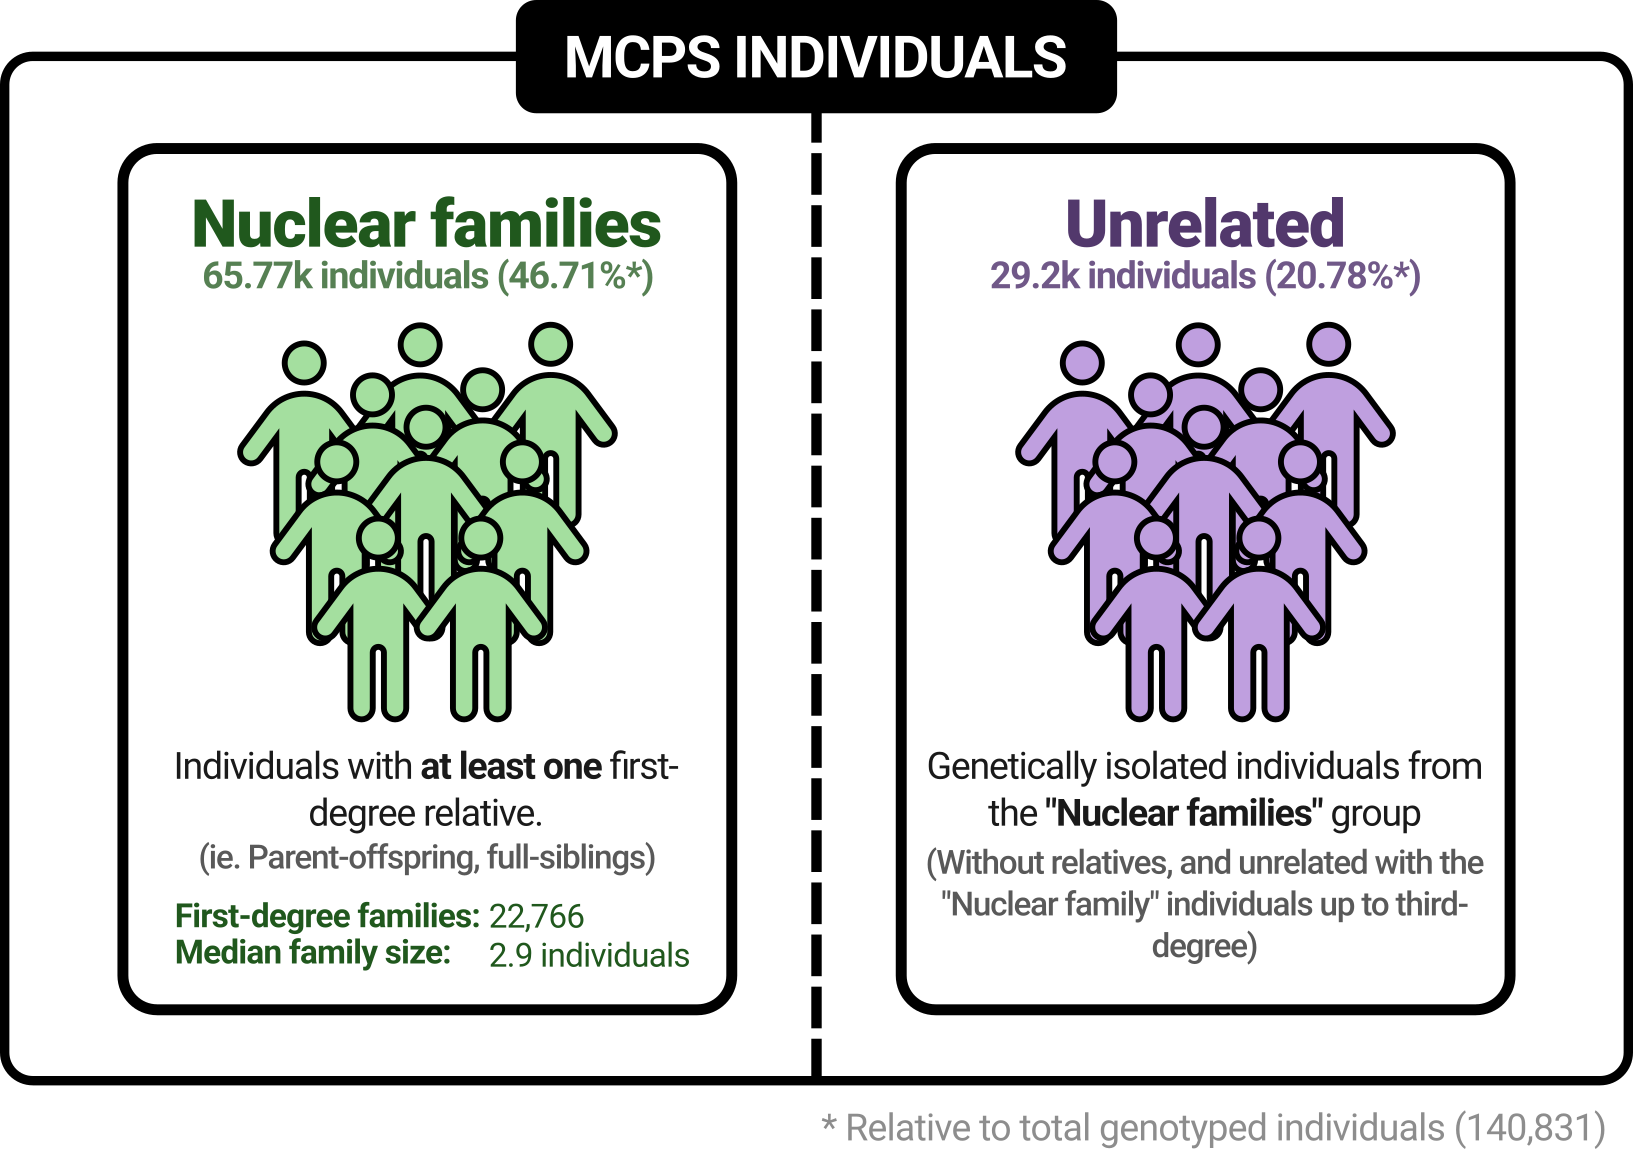
\includegraphics[width=0.90\textwidth]{img/diagrams/unrelated-individuals.png}
%     \end{column}
%   \end{columns}
% \end{frame}